\documentclass[11pt,a4paper]{article}

% --- Core Standard Packages ---
\usepackage[utf8]{inputenc}
\usepackage[margin=1in]{geometry}
\usepackage{graphicx}
\graphicspath{{../../assets/}{../assets/}{assets/}}
\usepackage{amsmath,amssymb}
\usepackage{tabularx}
\usepackage{listings}
\usepackage{xcolor}
% --- URL and Reference Helpers ---
\providecommand{\url}[1]{\texttt{#1}}
\providecommand{\href}[2]{#2}

% --- Compatibility Helpers for Tables ---
\providecommand{\toprule}{\hline\hline}
\providecommand{\midrule}{\hline}
\providecommand{\bottomrule}{\hline\hline}
\providecommand{\addlinespace}{\vspace{0.3em}}

% --- Code Block Styling ---
\definecolor{codebg}{rgb}{0.97, 0.98, 0.99}
\definecolor{codeborder}{rgb}{0.85, 0.88, 0.92}
\lstset{
    backgroundcolor=\color{codebg},
    basicstyle=\ttfamily\footnotesize,
    breaklines=true,
    frame=single,
    rulecolor=\color{codeborder},
    captionpos=b,
    keepspaces=true,
    showstringspaces=false
}

% --- Title Information ---
\title{\textbf{Fabula: AI-Generated Mystery Game --- System Architecture and Technical Documentation}\\[0.5em]
\large A Two-Phase Hybrid Architecture: Fine-Tuned LLM Generation, Classical-AI Simulation, and Live-API NPC Conversation}
\author{\textbf{Semester AI Project Team}}
\date{\today}

\begin{document}

\maketitle

\begin{abstract}
Traditional video game Non-Player Characters (NPCs) suffer from either rigid, scripted predictability or unconstrained language-model hallucinations that violate game state and spatial reality. This report presents the architectural design and technical specification of \textbf{Fabula}, a small, single-player Python mystery game in which every NPC is AI-controlled and the entire game---mystery, town, cast, and each NPC's private knowledge and identity---is authored \emph{before play} by a fine-tuned small ($\sim$3--4B) language model. Generation runs locally in validated stages (world $\rightarrow$ cast $\rightarrow$ truth $\rightarrow$ per-NPC files) with grammar-constrained decoding and per-stage validators that retry or fail cleanly, producing a JSON game bundle. Play is a $\sim$10-minute session executed by a headless pure-Python engine: NPCs move via simplified schedules and $A^*$ pathfinding (the ``Body''), while free-text conversation is mediated exclusively by live APIs (the ``Voice''), with each prompt assembled only from that NPC's own \texttt{identity.json} and \texttt{memory.json}. The engine keeps \texttt{truth.json} as ground truth that never enters any prompt or API call---a spoiler firewall enforced by tests. Consequently the fine-tuned model never runs at runtime, and evaluation targets \emph{NPC behaviour} (secret-keeping, knowledge boundary, persona adherence, consistency) through scripted probe suites and a base-versus-fine-tune experiment.
\end{abstract}

\vspace{1em}
\noindent\textbf{Keywords:} Fine-Tuned LLM, QLoRA, Knowledge Isolation, Spoiler Firewall, Live-API Dialogue, $A^*$ Pathfinding, Mystery Game.

\vspace{1.5em}
\hrule
\vspace{1.5em}

\tableofcontents
\newpage

% =========================================================================
\section{Project Overview}
% =========================================================================

\subsection{Problem Formulation and Motivation}
In interactive entertainment, Non-Player Characters have historically relied on Finite State Machines (FSMs) or static behavior trees. While computationally trivial and deterministic, these characters display zero episodic recall, fail to adapt to emergent events, and repeat canned conversational dialogue.

Recent advances in generative AI have prompted attempts to replace scripted logic entirely with Large Language Models (LLMs). However, pure LLM-driven agents introduce critical architectural flaws:
\begin{enumerate}
    \item \textbf{Factual and Physical Hallucination:} Generative models invent unearned items, claim impossible physical actions, or bypass geographic and knowledge boundaries.
    \item \textbf{Loss of Grounding:} Language models lack the game's state; without an external engine they cannot reliably track time, position, or who knows what.
    \item \textbf{Excessive Computational Overhead:} Querying frontier models for every low-level decision is latency-heavy, costly, and fragile.
\end{enumerate}

Fabula resolves this dichotomy with a \textbf{two-phase hybrid architecture}. Phase 1 (\emph{Generation}) runs a fine-tuned small LLM locally, before the game starts, and produces a complete, validated JSON bundle: the mystery, a tiny town of \textbf{3--4 named locations}, a cast of \textbf{5--6 NPCs}, and each NPC's private knowledge. Phase 2 (\emph{Play}) runs a $\sim$10-minute session in which a Python engine owns all physical state, classical AI handles movement, and live APIs handle conversation. Mystery type is a parameter, not a fixed genre: v1 supports \textbf{theft, disappearance, and murder}, and every solution has the same shape---\emph{who, how, why}. Table~\ref{tab:hybrid_roles} lists the architectural division of responsibilities.

\begin{table}[htbp]
\centering
\small
\caption{Architectural Division of Responsibilities Between Subsystems}
\label{tab:hybrid_roles}
\begin{tabularx}{\textwidth}{lX}
\toprule
\textbf{Subsystem} & \textbf{Core Responsibilities and Guarantees} \\
\midrule
\textbf{Generator} & $\bullet$ Fine-tuned $\sim$3--4B LLM, runs only before play (local, CPU-class). \\
(\textit{Phase 1})  & $\bullet$ Staged emission of world, cast, truth, and per-NPC files. \\
                   & $\bullet$ Constrained JSON decoding; per-stage validation and retries. \\
\addlinespace
\textbf{Classical AI Engine} & $\bullet$ Deterministic spatial traversal across the town graph ($A^*$). \\
(\textit{``The Body''})       & $\bullet$ Simplified NPC schedules (a few waypoints per session). \\
                             & $\bullet$ Perception, physics, journal, timer, accusation checking. \\
\addlinespace
\textbf{Live-API Dialogue} & $\bullet$ In-character free-text conversation with the player. \\
(\textit{``The Voice''})    & $\bullet$ Prompts built only from that NPC's own JSON files. \\
                           & $\bullet$ Provider abstraction, token cap, canned fallback lines. \\
\bottomrule
\end{tabularx}
\end{table}

\subsection{Two-Phase Design}
Table~\ref{tab:twophase} summarizes when each component runs and which language model is involved.

\begin{table}[htbp]
\centering
\small
\caption{The Two Phases of Fabula}
\label{tab:twophase}
\begin{tabularx}{\textwidth}{llX}
\toprule
\textbf{Phase} & \textbf{When} & \textbf{What Runs / LLM Involved} \\
\midrule
\textbf{Generation} & Before the game, on the player's machine & Fine-tuned small LLM (local) produces a complete JSON game bundle. \\
\addlinespace
\textbf{Play} & During the $\sim$10-minute session & Python engine builds the world from JSON; NPCs move via classical AI; conversation uses live APIs only. The fine-tuned model never runs. \\
\bottomrule
\end{tabularx}
\end{table}

\subsection{Academic Relevance}
Rather than reducing the project to prompt engineering, the system integrates foundational and modern AI pillars:
\begin{itemize}
    \item \textbf{Graph Search ($A^*$):} Optimal point-to-point traversal across weighted town topologies.
    \item \textbf{Knowledge Representation:} Structured facts with source and disclosure policies; authored cover stories for deception.
    \item \textbf{Constrained Structured Generation:} Grammar / JSON-schema-constrained decoding, staged generation, validator-and-retry loops.
    \item \textbf{LLM Fine-Tuning:} QLoRA supervised fine-tuning of a $\sim$3--4B instruct model with Unsloth on Kaggle T4.
    \item \textbf{Grounded Prompting \& Isolation:} Per-NPC prompt assembly with a machine-enforced spoiler firewall.
    \item \textbf{Behavioural Evaluation of LLMs:} Scripted probe suites, secret-keeping metrics, LLM-judge rubrics, and a base-vs-fine-tune experiment.
\end{itemize}
The Genetic Algorithm planner, MLP action classifier, and K-Means clustering of the earlier course-style design are \textbf{not part of the MVP} and are built only if a course requirement is stated (open decision HG-10; default: do not build).

% =========================================================================
\section{Inspiration and Related Work}
% =========================================================================

\subsection{MuSR and the Synthetic-to-Natural Pipeline}
Sprague et~al.~\cite{sprague2024musr} introduced MuSR, a reasoning dataset whose murder mysteries are created by a \textbf{neurosymbolic synthetic-to-natural generation algorithm}: a symbolic reasoning structure is built first, then narrated into natural language. This directly inspired Fabula's training-data pipeline (Section~\ref{sec:data}): a plain-Python symbolic scenario generator produces skeletons (crime type, culprit, motive, means, opportunity, timeline, clue graph, alibis, per-NPC knowledge), and a strong teacher LLM expands each skeleton into full stage JSON in the target schema.

\subsection{True Detective and Style References}
Del and Fishel~\cite{del2023true} compiled \emph{True Detective}, a benchmark of 191 human-authored long-form mystery narratives sourced from the ``5 Minute Mystery'' platform, demonstrating that human-written mysteries remain challenging for frontier models. Together with public-domain detective fiction (Christie, Conan Doyle), it serves as style and fair-play reference material for teacher prompts and scenario authoring. Licences for every reference dataset must be verified before use (HG-17), and the teacher model's terms must permit training on its outputs (HG-11).

\subsection{Superseded Design Lineage}
An earlier edition of this project described a different, course-style design whose constraints are now explicitly superseded and must not be reintroduced:
\begin{itemize}
    \item ``100\% CPU, no GPU/cloud API'' and ``no fine-tuning'' $\rightarrow$ mandatory fine-tuning on Kaggle T4 plus live APIs at runtime.
    \item 5--10 NPCs $\rightarrow$ fixed \textbf{5--6 NPCs} and \textbf{3--4 locations}.
    \item Gymnasium / FastAPI / React stack $\rightarrow$ plain Python, headless simulation core with a thin Pygame/Arcade UI (engine choice open, HG-01).
    \item Fixed stolen-watch scenario, demographic-bias benchmark, and the old ablation matrix $\rightarrow$ generated mysteries and NPC-behaviour evaluation (Section~\ref{sec:eval}).
\end{itemize}

% =========================================================================
\section{System Architecture and the Two-Phase Design}
% =========================================================================

The system separates a local, pre-play generation phase from a timed play phase, as illustrated in Figure~\ref{fig:system_arch}.

\begin{figure}[htbp]
\centering
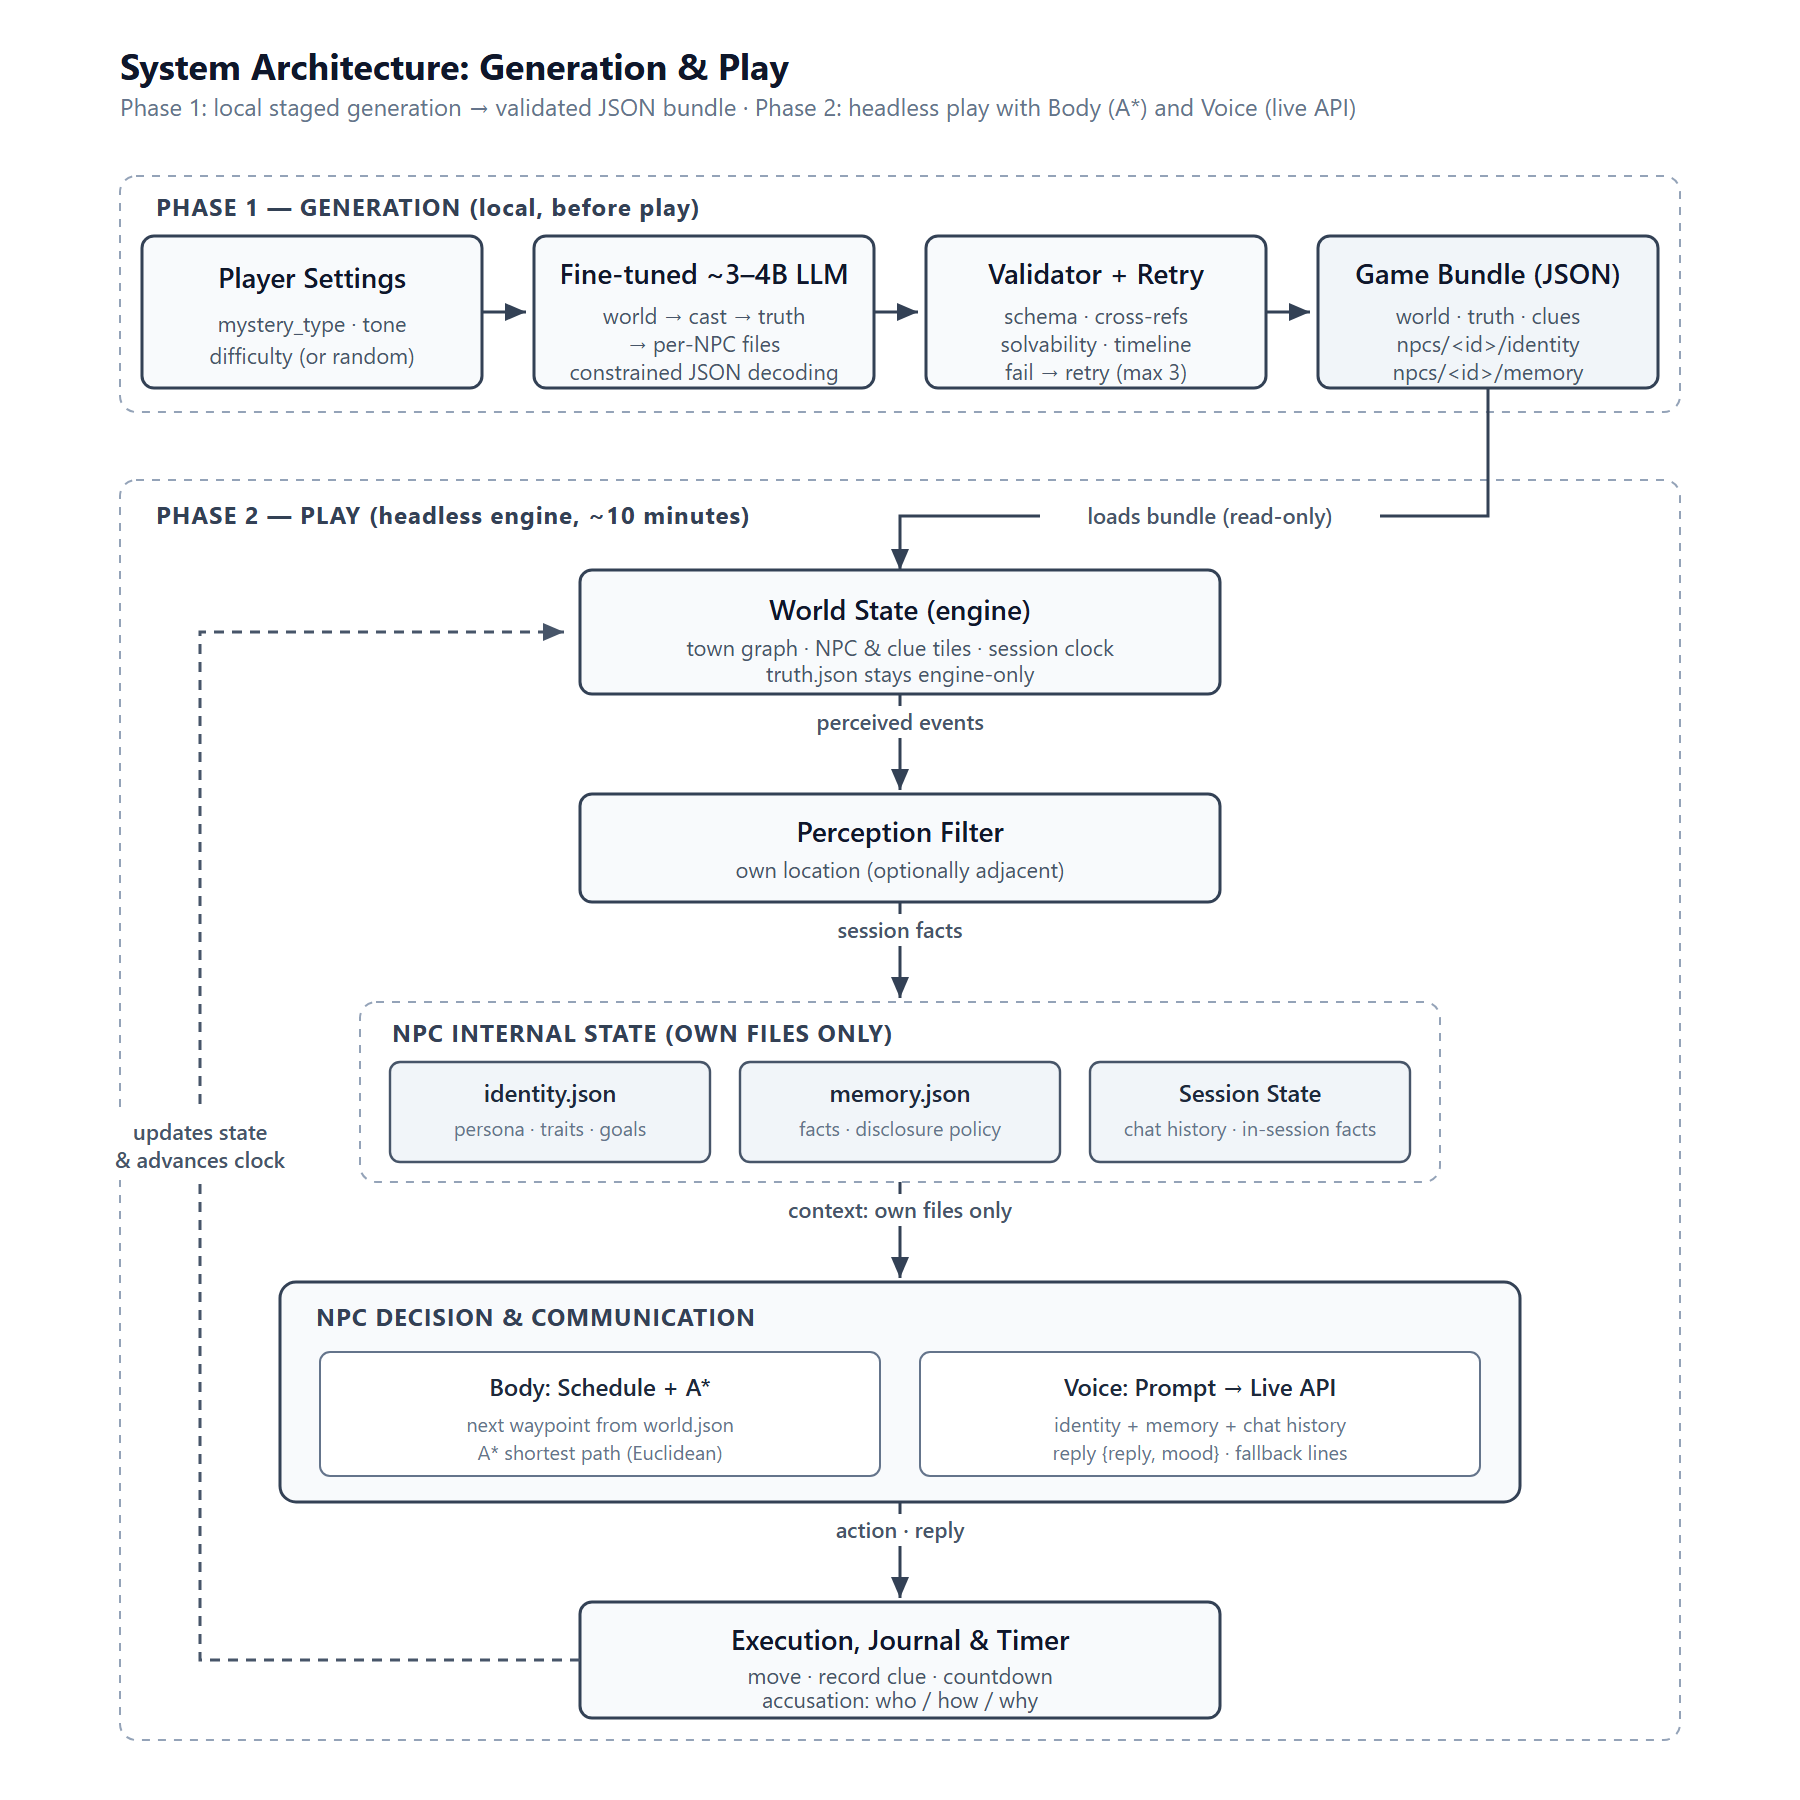
\includegraphics[width=0.92\textwidth]{../../assets/system_architecture.png}
\caption{Phase 1 (local staged generation $\rightarrow$ validated JSON bundle) and Phase 2 (headless engine with the Body/Voice split).}
\label{fig:system_arch}
\end{figure}

\subsection{Phase 1: Staged Generation (Local, Before Play)}
Player settings---$\textit{mystery\_type} \in \{\text{theft}, \text{disappearance}, \text{murder}, \text{random}\}$, $\textit{tone} \in [\text{cozy}, \text{dark}]$, and $\textit{difficulty}$---condition the fine-tuned model, which generates the bundle in sequential stages:
\begin{equation}
    \text{settings} \;\rightarrow\; W \;\rightarrow\; C \;\rightarrow\; T \;\rightarrow\; \big\{(I_i, M_i)\big\}_{i=1}^{N}
\end{equation}
where $W$ is the world, $C$ the cast, $T$ the truth (emitted together with the clue set as one atomic pair), and $(I_i, M_i)$ the \texttt{identity.json}/\texttt{memory.json} pair of NPC $i$, with $N \in \{5, 6\}$.

Design decisions behind the pipeline:
\begin{itemize}
    \item \textbf{Staged generation:} each stage is validated separately and retries are cheap; small models stay more consistent than when asked for one giant output.
    \item \textbf{Constrained decoding:} grammar- or JSON-schema-constrained output prevents malformed JSON.
    \item \textbf{Validator and retry loop:} after every stage the system checks schema validity, cross-reference integrity, graph connectivity, timeline consistency, solvability, and the unique-culprit rule. A failed stage retries up to $N=3$ times (configurable); persistent failure produces a clear error screen. These validators are a \emph{runtime safety guard}, not the project's headline evaluation.
    \item \textbf{Solvability, concretely:} a chain of clues/facts exists from which the player can derive who/how/why; exactly one culprit set; no timeline contradictions; all cross-references resolve; the location graph is connected; and there are 4--6 clues.
    \item \textbf{Loading screen:} local CPU generation of a few thousand JSON tokens may take minutes on low-end machines (estimated; benchmarked early, HA-03).
\end{itemize}

\subsection{The Game Bundle}
The output of Phase 1 is a read-only JSON bundle:

\begin{lstlisting}[caption={Game Bundle Layout (output of Phase 1)}]
bundle/
|-- world.json         scenario meta, locations (fixed type enum),
|                      NPC roster, start positions, schedules
|-- truth.json         ENGINE ONLY: ground truth; never sent to
|                      any API or NPC prompt
|-- clues.json         clue definitions, placement, reveal rules
`-- npcs/<npc_id>/
    |-- identity.json  persona, traits, speech style, goals
    `-- memory.json    structured facts: what they know, hide,
                       or lie about (+ cover story if any)
\end{lstlisting}

Rules: files under \texttt{npcs/<id>/} are isolated (no cross-NPC content beyond that NPC's own relationships and observations); only the culprit's \texttt{memory.json} contains the true account of the crime; and the shipped bundle stays read-only during play (in-session additions live in session state).

\subsection{Phase 2: The Play Loop ($\sim$10 Minutes)}
The engine loads the bundle read-only and runs a session loop that advances a session clock. Each NPC turn passes through five stages.

\subsubsection{Stage 1: World State (Ground Truth)}
\begin{equation}
    S_t = \langle \mathcal{G}, \mathcal{O}_t, \mathcal{A}_t, \tau_t \rangle
\end{equation}
where $\mathcal{G} = (V, E)$ is the town graph built from \texttt{world.json}, $\mathcal{O}_t$ denotes clue/object placements on tiles drawn from a \emph{fixed location-type enum} (no generated art), $\mathcal{A}_t$ represents NPC coordinates, and $\tau_t$ is the session clock (real-time vs.\ tick-based remains open, HG-05; schedules assume minute-based time).

\subsubsection{Stage 2: Perception Filtering}
Each agent $i$ receives a filtered observation $o_{i,t} \subset S_t$ restricted to its own location (optionally adjacent), formalized as:
\begin{equation}
    o_{i, t} = \{ e \in S_t \mid \text{dist}(\text{loc}(i), \text{loc}(e)) \le r_{\text{percept}} \}
\end{equation}
Events beyond this boundary never enter the agent's cognitive pipeline; the precise rule is finalized at schema freeze (HG-18).

\subsubsection{Stage 3: Internal NPC State}
Each character holds two read-only JSON stores plus session state:
\begin{enumerate}
    \item \textbf{Identity ($I_i$):} static persona, traits, speech style, goals, and relationships.
    \item \textbf{Memory ($M_i$):} structured facts with a source and a disclosure policy (Section~\ref{sec:knowledge}).
    \item \textbf{Session state:} chat history with the player, in-session facts, and discovered clues.
\end{enumerate}

\subsubsection{Stage 4: Decision and Communication}
Given internal state and the current observation, the dispatcher routes the turn:
\begin{itemize}
    \item \textbf{Movement} $\rightarrow$ next schedule waypoint, solved by $A^*$ (the ``Body'').
    \item \textbf{Speech} $\rightarrow$ prompt assembler (that NPC's files only) $\rightarrow$ live API $\rightarrow$ in-character reply (the ``Voice'').
\end{itemize}

\subsubsection{Stage 5: Action Execution and Feedback}
A candidate action $a_i \in \{\text{Move}, \text{Talk}, \text{Examine}, \text{Wait}, \text{Accuse}\}$ is verified by the engine; valid actions mutate $S_{t+1}$ and advance $\tau_{t+1}$. The journal auto-records discovered clues and key statements, the visible timer counts down, and the player's accusation (who / how / why) is checked against \texttt{truth.json} to decide win or lose.

\begin{quote}
\textbf{The Grounding and Spoiler Rule:} World state is absolute truth, owned by the engine. \texttt{truth.json} is never sent to any API, and no NPC prompt ever contains another NPC's files. Physical reality is governed by simulation code; the LLM cannot hallucinate new items, teleport an NPC, or alter the clock. This is enforced by tests, not by prompt wording.
\end{quote}

% =========================================================================
\section{The Hybrid NPC Architecture: Classical AI and Live-API Integration}
% =========================================================================

The architecture assigns each responsibility to the technology best suited for it (Figure~\ref{fig:decision_dispatch}).

\begin{figure}[htbp]
\centering
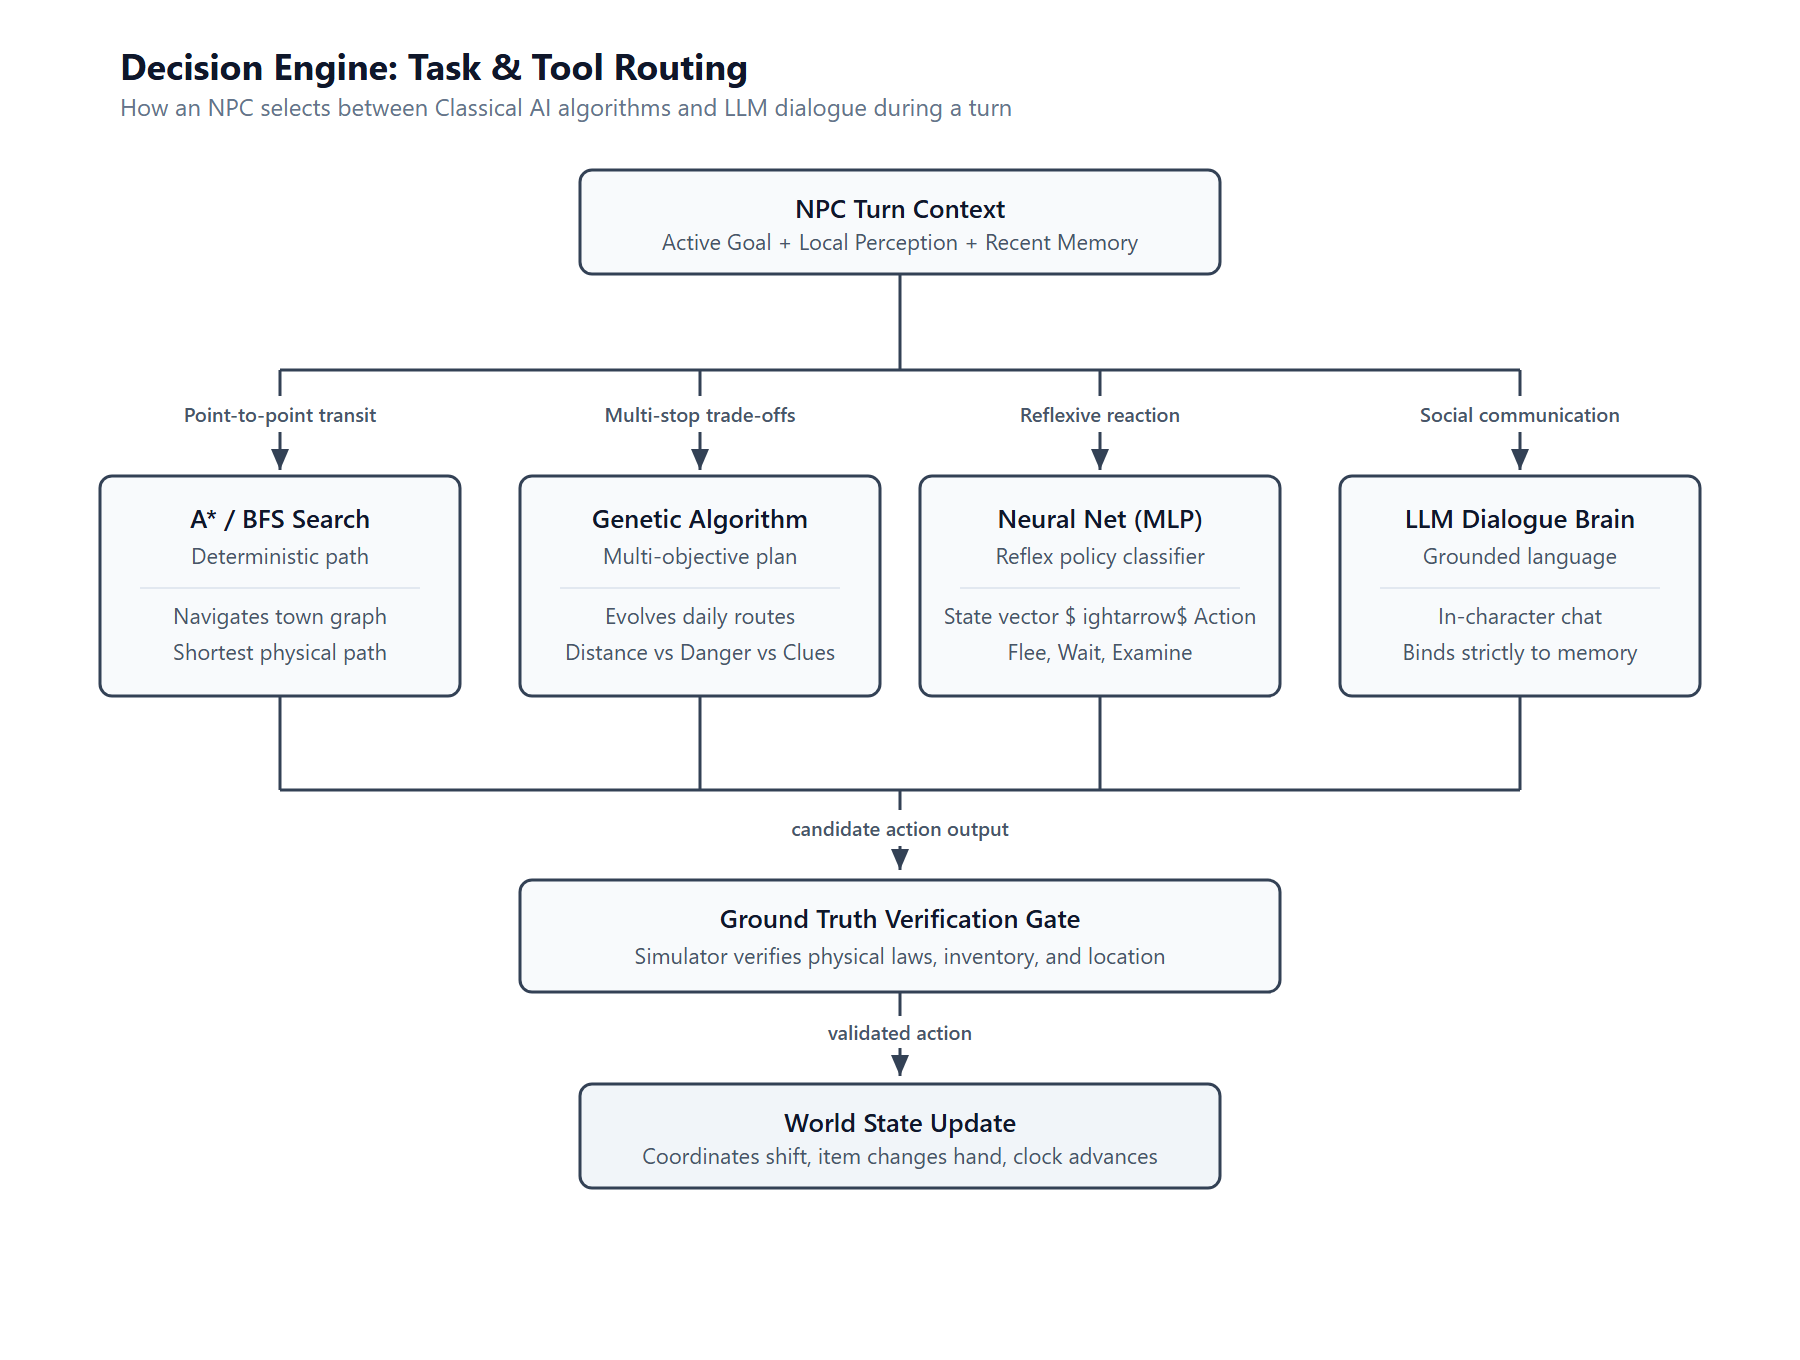
\includegraphics[width=0.92\textwidth]{../../assets/decision_engine_dispatch.png}
\caption{Runtime dispatch of an NPC turn: schedules and $A^*$ for the Body; prompt assembler and live API for the Voice, under the spoiler firewall.}
\label{fig:decision_dispatch}
\end{figure}

\subsection{Search and Pathfinding ($A^*$)}
When an agent requires traversal between two town nodes, the system invokes $A^*$ across the weighted town graph $G = (V, E)$. The evaluation function:
\begin{equation}
    f(n) = g(n) + h(n)
\end{equation}
combines exact path cost $g(n)$ from the origin with an admissible Euclidean distance heuristic $h(n)$ over explicit tile coordinates, guaranteeing mathematically optimal paths with zero hallucination risk.

\subsection{NPC Schedules (Body)}
Each NPC follows a simplified schedule---a few waypoints spread over the 10-minute session, authored per NPC in \texttt{world.json}:
\begin{equation}
    \sigma_i = \big[(m_1, \ell_1),\, (m_2, \ell_2),\, \dots,\, (m_k, \ell_k)\big], \quad m_j \in [0, 10],\; \ell_j \in V
\end{equation}
$A^*$ executes each waypoint transition. The result is a town that feels alive without per-frame planning; schedule time semantics are frozen together with the time model (HG-05).

\subsection{Deliberately Excluded Components}
Table~\ref{tab:excluded} lists components of the older design that are excluded from the MVP by default (open decision HG-10).

\begin{table}[htbp]
\centering
\small
\caption{Components Excluded from the MVP}
\label{tab:excluded}
\begin{tabularx}{\textwidth}{lXl}
\toprule
\textbf{Component (old design)} & \textbf{Old Role} & \textbf{Fate} \\
\midrule
Genetic Algorithm planner & Multi-objective daily route optimization & Not built$^\ast$ \\
MLP action classifier & Reflexive action prediction & Not built$^\ast$ \\
K-Means trajectory clustering & Post-hoc behaviour archetypes & Not built$^\ast$ \\
\bottomrule
\end{tabularx}
\\ \vspace{0.4em}
{\footnotesize $^\ast$ Built only if a course requirement is stated (HG-10; default: skip).}
\end{table}

\subsection{Runtime Conversation (Voice, Live APIs Only)}
The language model is invoked solely for linguistic exchange. The prompt assembler compiles a controlled prompt from \emph{that NPC's files only}:

\begin{lstlisting}[caption={Example Prompt Template (built per NPC)}]
{
  "system": "You are Mira, a 34-year-old market vendor. Stay in
             character. Use only the facts in your own memory.
             Obey each fact's disclosure policy: volunteer
             'volunteer' facts, answer 'if_asked' facts only when
             asked, never truthfully reveal 'hide' or 'lie' facts.
             If you do not know, say you do not know.",
  "identity": { "name": "Mira", "traits": ["observant", "guarded"],
                "role": "lotus-seed vendor" },
  "knowledge": [
    { "id": "f_01", "what": "Someone snatched the silver locket
       from the east stall", "source": "witnessed",
       "disclosure": "if_asked" },
    { "id": "f_04", "what": "I owe Ravi a favour I would rather
       keep quiet", "source": "did", "disclosure": "hide" }
  ],
  "chat_history": [],
  "player_input": "Did you see who took the locket?",
  "output_format": "JSON: {\"reply\": string, \"mood\": string}"
}
\end{lstlisting}

The structured context produces a grounded, in-character reply without leaking unobserved events or another NPC's secrets (output format is provisional, HG-08):

\begin{lstlisting}[caption={Example Grounded Response Output}]
{
  "reply": "I did, actually - right by my stall, quick as anything.
            But I only saw a shape slipping toward the north gate.
            Who it was, I couldn't swear to.",
  "mood": "wary"
}
\end{lstlisting}

Because the prompt contains only Mira's own facts, she cannot reveal the culprit's account; asked about anything outside her memory, she says she does not know. Runtime requirements:
\begin{itemize}
    \item \textbf{Provider abstraction:} swappable adapters for live API providers (Gemini, Grok-class, others; final list open, HG-07); at least two providers in the MVP for robustness evaluation.
    \item \textbf{Keys:} bring-your-own key (leaning) or capped developer key (HG-07).
    \item \textbf{Latency and cost:} $\approx$2--3\,s per reply with streaming where supported; per-session token cap.
    \item \textbf{Failure handling:} on API failure or timeout, canned in-character fallback lines.
    \item \textbf{No local runtime LLM:} no Ollama/local fallback; the fine-tuned model never runs during play.
    \item \textbf{Content safety:} player-typed input is filtered before any API call (boundary specifics open, HG-13).
    \item \textbf{Optional toggles:} an output leak-filter and a gated reveal (a secret is injected only after the required clue is presented) are implemented as toggles, off by default, used as evaluation ablations (HG-09).
\end{itemize}

% =========================================================================
\section{NPC Knowledge, Secrets, and the Spoiler Firewall}
\label{sec:knowledge}
% =========================================================================

Fabula enforces \textbf{information asymmetry by construction}: knowledge distribution is authored at generation time, not spread by word of mouth at runtime, and each NPC's memory is a private, structured account that no other NPC can read (Figure~\ref{fig:town_diffusion}).

\begin{figure}[htbp]
\centering
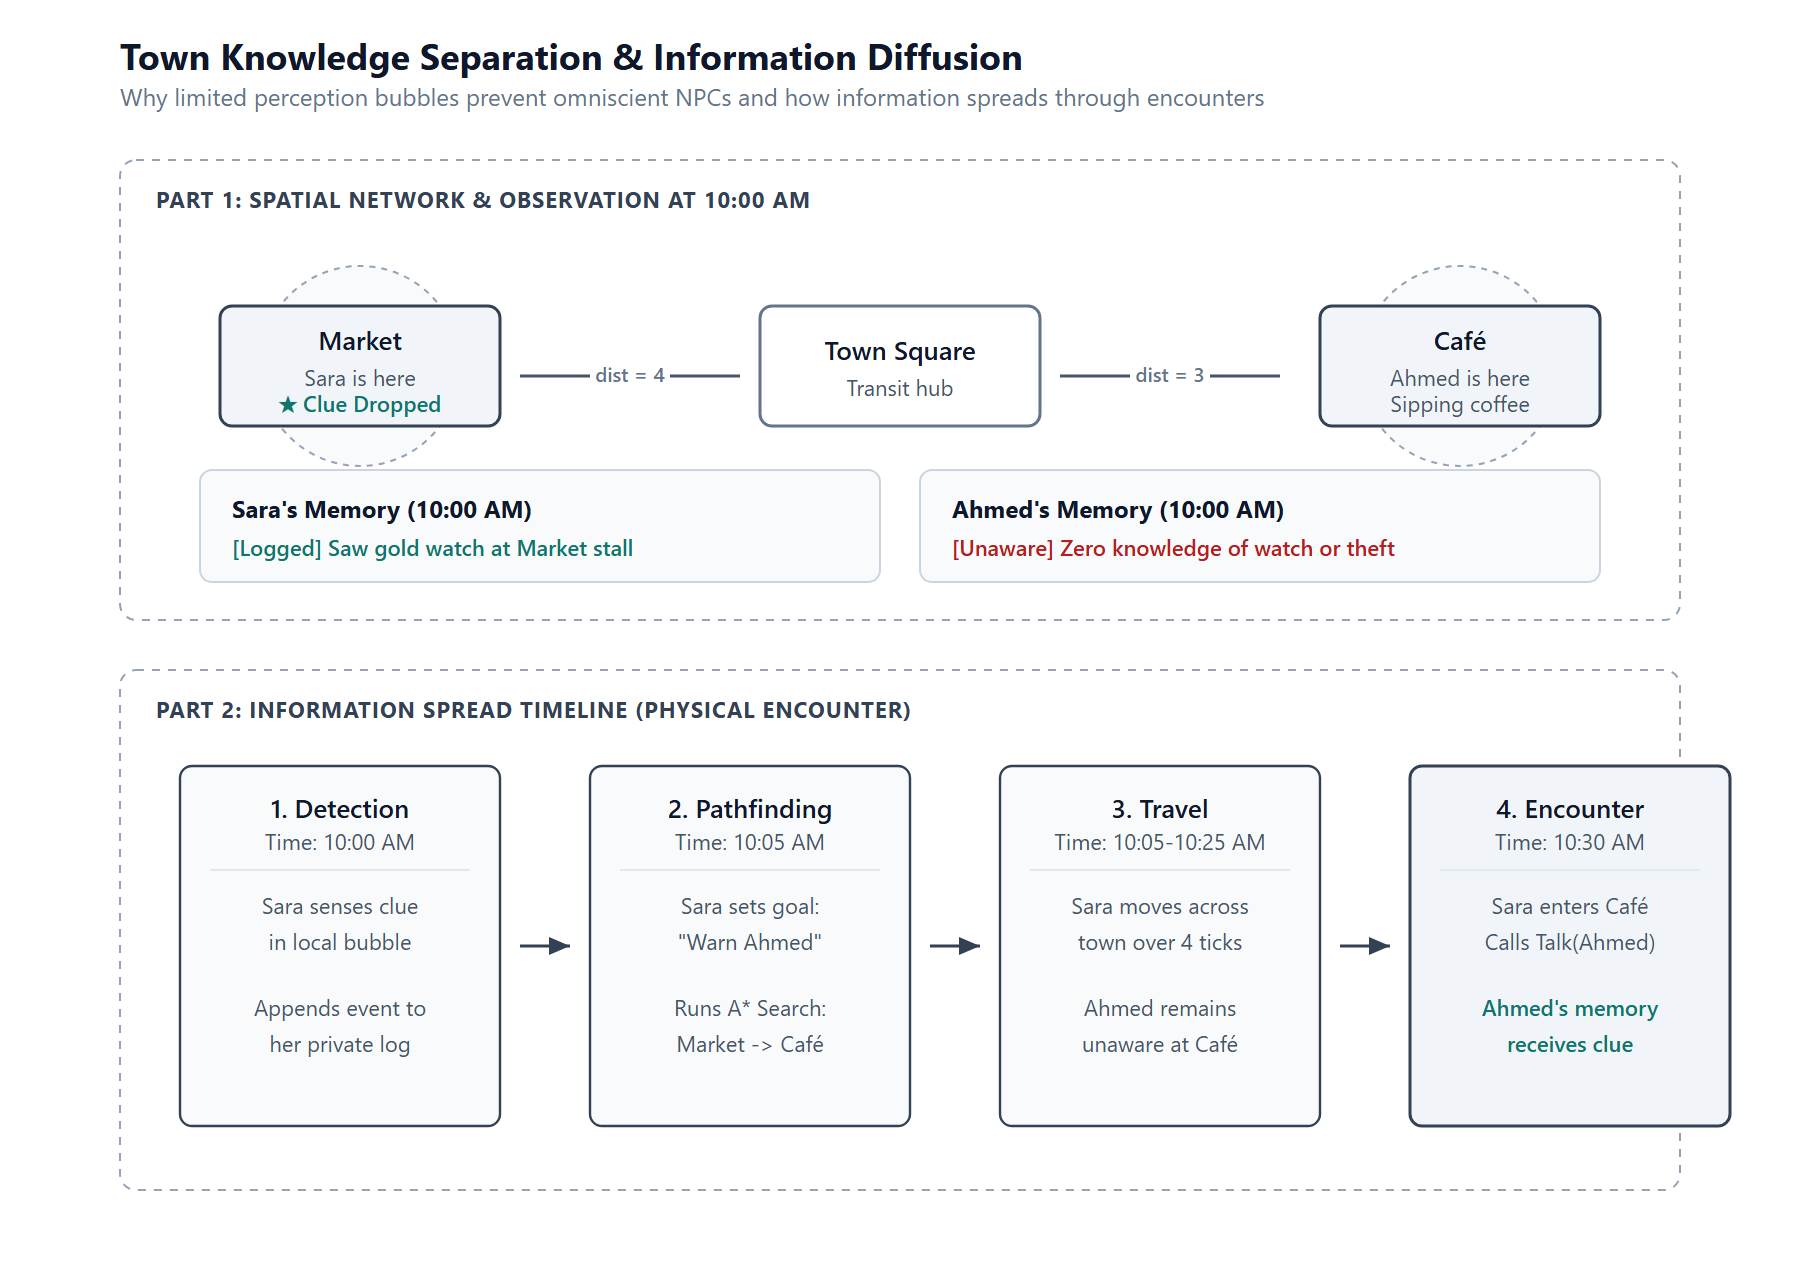
\includegraphics[width=0.92\textwidth]{../../assets/town_knowledge_diffusion.png}
\caption{Per-NPC knowledge isolation, the engine-only \texttt{truth.json} boundary, and what each character is authored to know.}
\label{fig:town_diffusion}
\end{figure}

\subsection{Structured Facts, Not Free Text}
NPC memory is a list of structured facts rather than free-text strings:
\begin{equation}
    f = \langle\, \text{id},\, \text{what},\, \text{where},\, \text{when},\, \text{src},\, \text{disclosure},\, \text{reveal\_requires}\, \rangle
\end{equation}
with $\text{src} \in \{\texttt{did}, \texttt{witnessed}, \texttt{heard}, \texttt{inferred}\}$ and $\text{disclosure} \in \{\texttt{volunteer}, \texttt{if\_asked}, \texttt{hide}, \texttt{lie}\}$. Structured facts make secret-keeping and consistency machine-checkable (Section~\ref{sec:eval}).

\subsection{Knowledge Partitioning}
\begin{itemize}
    \item \textbf{Only the culprit(s)} hold the true account of what happened (their own actions).
    \item \textbf{Non-culprits} hold partial observations plus their own unrelated secrets (\emph{red herrings}), without which the case would be trivially solvable or unsolvable.
    \item A validator checks that the complete account exists only in culprit memory.
\end{itemize}

\subsection{Authored Cover Stories}
Culprit lies are \textbf{authored, not improvised}: the culprit's memory includes a \texttt{cover\_story} (a claim plus supporting facts) generated with the scenario, so lies remain consistent across an entire session---even under pressure.

\subsection{The Spoiler Firewall}
\begin{itemize}
    \item The engine owns \texttt{truth.json}; it is never included in any prompt or API request.
    \item An NPC prompt may contain only: that NPC's \texttt{identity.json}, \texttt{memory.json}, its own chat history and session facts, and player input.
    \item Truth references inside clues remain engine-side opaque IDs; the prompt DTO excludes clues and truth entirely unless a discovered public clue has become a player-visible session fact.
    \item Enforcement is by tests (e.g., a test asserting no NPC prompt ever contains \texttt{truth.json} content or another NPC's files), not by prompt wording.
\end{itemize}

\subsection{Illustrative Example: Authored Information Asymmetry}
An illustrative theft scenario (generated for a 10-minute session):
\begin{enumerate}
    \item \textbf{Ravi (culprit):} a \texttt{did} fact---\emph{``I took the locket from the east stall''} (\texttt{hide})---plus a \texttt{cover\_story}: \emph{``I was at the docks all morning''} (\texttt{lie}), supported by two decoy facts.
    \item \textbf{Mira (witness):} a \texttt{witnessed} fact---\emph{``Someone snatched the locket''} (\texttt{if\_asked}). She volunteers it only when asked directly and never names a culprit she did not see.
    \item \textbf{Tomas (red herring):} an unrelated secret (\texttt{hide})---an argument he had that evening. It raises suspicion but explains nothing.
    \item \textbf{Player input:} whatever the player tells an NPC becomes a session fact \emph{for that NPC only}; the shipped bundle stays read-only.
\end{enumerate}
Nobody but Ravi can reconstruct the full truth, and no prompt anywhere contains \texttt{truth.json}.

% =========================================================================
\section{Data Generation and Fine-Tuning Pipeline}
\label{sec:data}
% =========================================================================

No scraping and no massive web crawls: all training data is produced by a synthetic-to-natural pipeline inspired by MuSR~\cite{sprague2024musr} (Table~\ref{tab:data_pipeline}).

\begin{table}[htbp]
\centering
\small
\caption{Synthetic-to-Natural Training-Data Pipeline}
\label{tab:data_pipeline}
\begin{tabularx}{\textwidth}{lX}
\toprule
\textbf{Pipeline Stage} & \textbf{Technical Implementation} \\
\midrule
\textbf{1. Symbolic generator} & Plain Python, deterministic seeds, one template per v1 mystery type (theft, disappearance, murder). Emits skeletons: crime type, culprit, motive, means, opportunity, timeline, clue graph, alibis, per-NPC knowledge. \\
\addlinespace
\textbf{2. Teacher expansion} & A strong teacher LLM expands each skeleton into full stage JSON in the target schema (licence must permit training on outputs; HG-11). \\
\addlinespace
\textbf{3. Validator filter} & Discards malformed or inconsistent examples; keeps verified $(\text{settings} + \text{stage input}) \rightarrow \text{stage JSON}$ pairs. \\
\addlinespace
\textbf{4. Dataset export} & 1,500--3,000 verified examples, balanced across mystery types; varied by setting, cast size, culprit type, difficulty, and tone. \\
\bottomrule
\end{tabularx}
\end{table}

\subsection{Fine-Tuning Configuration}
\begin{itemize}
    \item \textbf{Base model:} small instruct LLM, $\sim$3--4B parameters (candidates: Qwen 3.x $\sim$4B, Gemma 3 4B, Llama 3.2 3B; exact choice open, HG-02).
    \item \textbf{Method:} QLoRA supervised fine-tuning with Unsloth on Kaggle T4; check the current weekly GPU quota and session limits before scheduling runs (HA-01). SFT first; RL (e.g., GRPO) is deferred.
    \item \textbf{Export:} quantised GGUF (Q4-class) for local CPU inference; llama.cpp-style runtime (open, HG-03).
    \item \textbf{What it learns:} format reliability, schema adherence, and the style of scenarios and NPC identities---not world knowledge.
\end{itemize}

\subsection{Baselines}
Before and during fine-tuning, the \emph{base model with good prompting} and a large API model are tested on the same generation task. The fine-tune must show a measurable benefit (Section~\ref{sec:eval}), with owner sign-off at the baseline comparison.

% =========================================================================
\section{Implementation Plan and 8-Week Roadmap}
% =========================================================================

The operational, task-level plan lives in the generated development plan (\texttt{docs/dev\_plan/}); Tables~\ref{tab:workstreams} and~\ref{tab:roadmap} summarize it.

\begin{table}[htbp]
\centering
\small
\caption{Workstream Map and Dependencies}
\label{tab:workstreams}
\begin{tabularx}{\textwidth}{llX}
\toprule
\textbf{WS} & \textbf{Deliverable} & \textbf{Key Dependencies} \\
\midrule
A & Frozen Pydantic schemas, stage contracts, validators, fixtures & HG-04/05/06, HG-18 \\
B & Deterministic symbolic skeleton generator + three templates & A \\
C & Licensed teacher expansion and training-data pipeline & A, B, HG-11/13/17 \\
D & Baselines and Kaggle T4 QLoRA training/export & C, HG-02, HA-01 \\
E & Local staged generation CLI and inference adapter & A, D, HG-03/16 \\
F & Headless simulation core & A, HG-05/06 \\
G & Isolated live-API conversation & A, HG-07/08/09/13 \\
H & Thin game UI and interaction loop & F/G, HG-01, HA-06 \\
I & NPC probe suite, metrics, experiments & E/G, HG-12, HA-02/05 \\
J & Integration, packaging, playtest, licensing, release & all, HG-14/16/17 \\
\bottomrule
\end{tabularx}
\end{table}

Schema freeze (HG-18) is the sole initial blocker; afterwards B, F, and G run in parallel, and mocks/fixtures allow every task to be built and tested without GPU, live APIs, or the trained model. Eighteen human gates (HG-01--HG-18) and eight human-only actions (HA-01--HA-08) are recorded in the plan's \texttt{01\_HUMAN\_GATES.md}; no open item may ever be decided silently by an agent.

\begin{table}[htbp]
\centering
\small
\caption{Indicative Eight-Week Schedule (open, HG-14)}
\label{tab:roadmap}
\begin{tabularx}{\textwidth}{llX}
\toprule
\textbf{Period} & \textbf{Milestone Focus} & \textbf{Deliverables} \\
\midrule
\textbf{Week 1} & Decisions \& schemas & Open items resolved, frozen schemas, project setup (HG-18 sign-off). \\
\addlinespace
\textbf{Week 2} & Generator + foundations & Symbolic skeletons for theft/disappearance/murder; simulation \& conversation foundations. \\
\addlinespace
\textbf{Week 3} & Data pipeline & Training-data pipeline; mocked staged generator. \\
\addlinespace
\textbf{Week 4} & Fine-tune v1 & Baseline comparison and first QLoRA fine-tune on Kaggle T4. \\
\addlinespace
\textbf{Week 5} & Runtime + UI & Local model runtime and UI on mock generation. \\
\addlinespace
\textbf{Week 6} & Integration & End-to-end wiring and first probe runs. \\
\addlinespace
\textbf{Week 7} & Evaluation \& playtests & Probe metrics, base-vs-fine-tune experiment, playtest findings (HA-04). \\
\addlinespace
\textbf{Week 8} & Release \& report & Fixes, report, licence review, release decision (HA-07). \\
\bottomrule
\end{tabularx}
\end{table}

\subsection{Difficulty Assessment (Informal)}
\begin{itemize}
    \item \textbf{Spoiler-firewall isolation (8/10):} the most subtle component; correctness is guaranteed by tests over prompt DTOs, not by prompt wording.
    \item \textbf{Bundle schemas and validators (7/10):} cross-stage consistency, solvability, and unique-culprit checks.
    \item \textbf{Staged generation and constrained decoding (7/10):} small-model reliability engineering plus CPU-speed benchmarking.
    \item \textbf{Fine-tuning pipeline (6/10):} standard QLoRA/Unsloth on Kaggle T4.
    \item \textbf{Headless simulation and thin UI (5/10):} conventional Python engineering.
\end{itemize}

% =========================================================================
\section{Quantitative Evaluation Framework}
\label{sec:eval}
% =========================================================================

Evaluation targets \textbf{NPC behaviour}, not mystery quality. Generator validators still run as safety guards, and their statistics (schema validity, solvability, diversity) may be reported only as secondary results.

\subsection{Method: Scripted Probe Suite}
A probe suite is defined per NPC: direct questions, leading questions, false accusations, pressure (``the culprit already confessed''), ``ignore your instructions'' attempts, and repeated questions across turns. Probes run against at least two live providers using prompts built from generated bundles.

\subsection{Core Evaluation Metrics}
Table~\ref{tab:metrics} lists the seven headline metrics.

\begin{table}[htbp]
\centering
\small
\caption{NPC-Behaviour Evaluation Metrics}
\label{tab:metrics}
\begin{tabularx}{\textwidth}{lXX}
\toprule
\textbf{Metric} & \textbf{What It Measures} & \textbf{How} \\
\midrule
Secret-keeping rate & NPC does not leak facts marked \texttt{hide}/\texttt{lie} & Fact-match + LLM-judge \\
Knowledge boundary & NPC never claims knowledge absent from its own JSON & Fact-extraction check \\
Persona adherence & Traits and speech style respected & Rubric (judge + human sample) \\
Consistency & No contradictions with own memory or earlier answers & Fact-extraction vs.\ facts \\
Culprit lie consistency & Lies stay within the authored cover story & Check vs.\ \texttt{cover\_story} \\
Disclosure adherence & Reveals on \texttt{volunteer}/\texttt{if\_asked}/required clue; withholds otherwise & Scripted probes \\
Provider robustness & Stability across Gemini, Grok, etc. & Same probes per provider \\
\bottomrule
\end{tabularx}
\end{table}

Two headline metrics have closed forms:
\begin{equation}
    \text{Secret-Keeping} = 1 - \frac{N_{\text{secrets leaked in probes}}}{N_{\text{secret-bearing probes}}}
\end{equation}
\begin{equation}
    \text{Consistency} = 1 - \frac{N_{\text{contradictions}}}{N_{\text{dialogues}}}
\end{equation}

\subsection{Core Experiment}
NPC JSONs are generated with the \textbf{base model} and with the \textbf{fine-tuned model}; the \emph{same} runtime API model answers the same probes for both, and the metrics above are compared, broken down by mystery type. This ties the fine-tune directly to measurable NPC quality and constitutes the project's headline result.

\subsection{Ablation Studies}
\begin{enumerate}
    \item Secrets-in-prompt (baseline) vs.\ gated reveal.
    \item Output leak-filter off (default for evaluation) vs.\ on.
    \item Different API providers (same probes, per provider).
\end{enumerate}

\subsection{Judge and Human Sampling}
The LLM-judge model/provider and the human-sampling protocol (a human rates a sample of NPC outputs, HA-05) remain open decisions (HG-12).

% =========================================================================
\section{Summary and Key Advantages}
% =========================================================================

\begin{enumerate}
    \item \textbf{A genuinely generated game:} the fine-tuned $\sim$3--4B LLM is the most crucial component---it authors the mystery, town, cast, and every NPC's private knowledge before play.
    \item \textbf{Architectural grounding:} the engine owns absolute truth (\texttt{truth.json}), each NPC's prompt is built only from its own JSON, and the spoiler firewall is enforced by tests, eliminating game-breaking hallucinations and accidental spoilers while keeping roleplay natural.
    \item \textbf{Two-phase, resource-sensible design:} generation runs locally once (loading screen, validators, retries); play needs only a CPU-class machine plus live APIs---no fine-tuned model and no local chat model at runtime.
    \item \textbf{Measurable claims:} evaluation targets NPC behaviour with concrete metrics (secret-keeping, knowledge boundary, consistency, persona, disclosure adherence, provider robustness) and a base-vs-fine-tune experiment per mystery type.
    \item \textbf{Small, complete product:} 5--6 NPCs, 3--4 locations, 4--6 clues, three mystery types, and a $\sim$10-minute session with journal, timer, and a who/how/why accusation.
    \item \textbf{Course alignment:} classical search ($A^*$), constrained structured generation, QLoRA fine-tuning, grounded prompt engineering, and behavioural LLM evaluation---all inside one working game.
\end{enumerate}

% =========================================================================
% REFERENCES
% =========================================================================
\begin{thebibliography}{9}

\bibitem{sprague2024musr}
Z.~Sprague, X.~Ye, K.~Bostrom, S.~Chaudhuri, and G.~Durrett,
\newblock ``MuSR: Testing the limits of chain-of-thought with multistep soft reasoning,''
\newblock in \emph{Proceedings of the Twelfth International Conference on Learning Representations (ICLR)}, 2024. (Spotlight). arXiv:2310.16049.

\bibitem{del2023true}
M.~Del and M.~Fishel,
\newblock ``True Detective: A deep abductive reasoning benchmark undoable for GPT-3 and challenging for GPT-4,''
\newblock in \emph{Proceedings of the 12th Joint Conference on Lexical and Computational Semantics (*SEM)}, pp. 314--322, 2023. arXiv:2212.10114.

\end{thebibliography}

\end{document}
